\documentclass[a4paper]{article}

%% Language and font encodings
\usepackage[brazil]{babel}
\usepackage[utf8x]{inputenc}
\usepackage[T1]{fontenc}

%% Sets page size and margins
\usepackage[a4paper,top=3cm,bottom=2cm,left=3cm,right=3cm,marginparwidth=1.75cm]{geometry}

%% Useful packages
\usepackage{amsmath}
\usepackage{graphicx}
\usepackage[colorinlistoftodos]{todonotes}
\usepackage[colorlinks=true, allcolors=blue]{hyperref}
\usepackage{ragged2e}
\usepackage{setspace}
\usepackage{enumitem}
\usepackage{float}
\usepackage{caption}
% \usepackage{biblatex}

\newcommand*{\Scale}[2][4]{\scalebox{#1}{$#2$}}%
\newcommand*{\Resize}[2]{\resizebox{#1}{!}{$#2$}}%

\title{Tubo de Pitot no túnel de vento}
\author{Nikolas Bernardes Vieira de Freitas}

\setlength{\parindent}{2em}
\renewcommand{\baselinestretch}{1.5}

\begin{document}
\maketitle

\section{Resumo}


\section{Introdução}

\section{Embasamento teórico}

\section{Materiais}
    \begin{enumerate}[label=(\roman*)]
        \item Sonda de pressão
        \item Túnel de vento
    \end{enumerate}

\section{Montagem}


\section{Procedimento}

\subsection{Condução do experimento}

 \subsection{Considerações sobre o procedimento}
  \begin{enumerate}
      \item
  \end{enumerate}


\section{Dados obtidos}
    Os dados obtidos durante o funcionamento do túnel de vento
    \begin{center}
          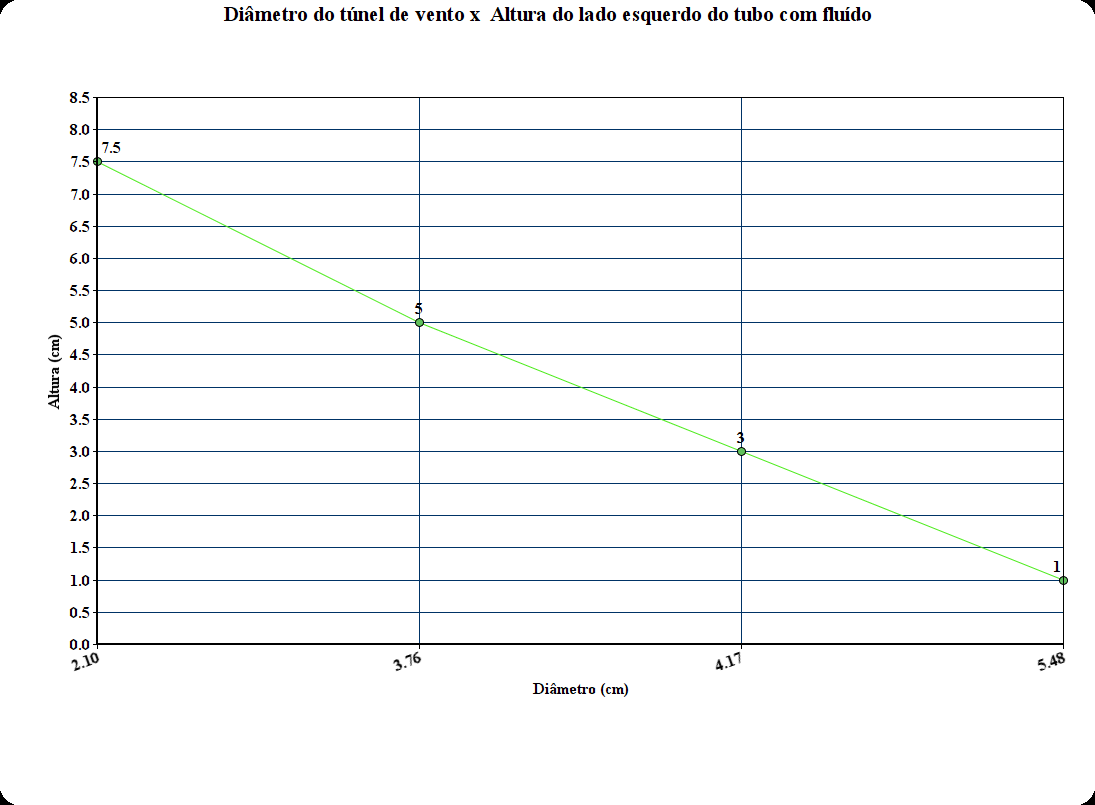
\includegraphics[width=\linewidth]{img/graphHeight.png}
          \label{graph}
    \end{center}


\section{Discussão dos dados}
    Segue as pressões calculadas para cada diâmetro do túnel de vento.
        \begin{center}
              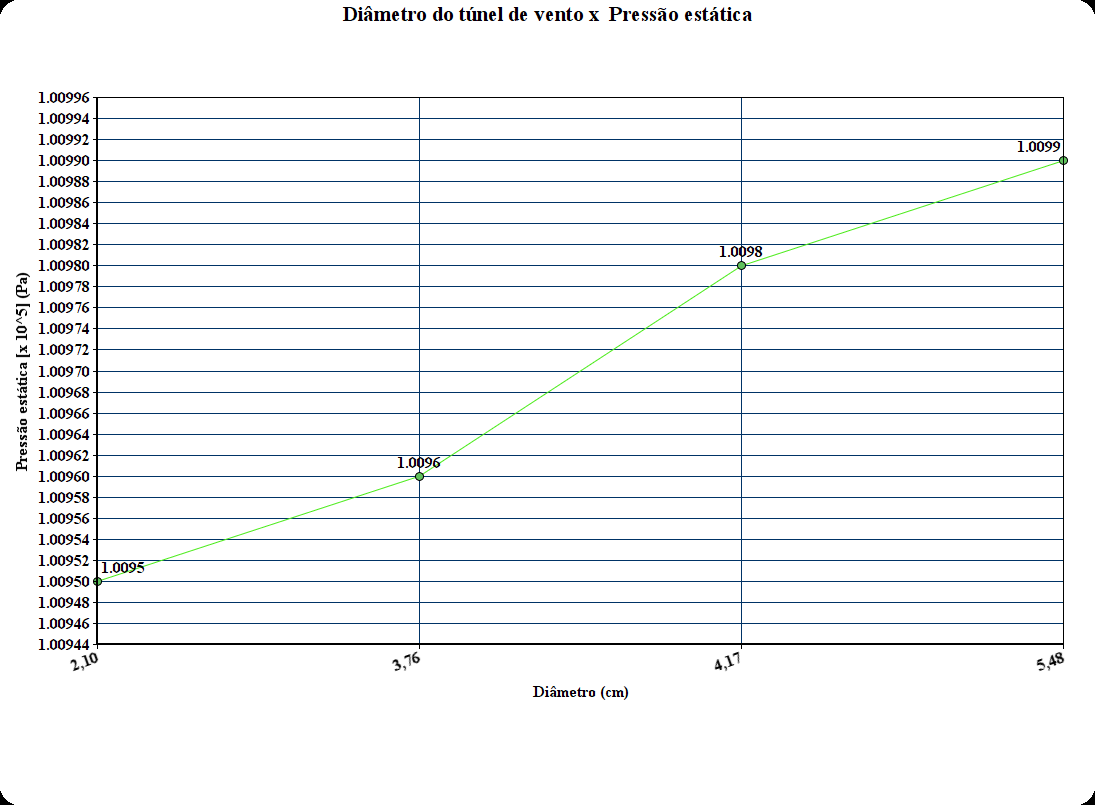
\includegraphics[width=\linewidth]{img/graphPression.png}
              \label{graph}
        \end{center}

\section{Conclusão}
    coisas aqui

\begin{thebibliography}{1}

\bibitem{knuthwebsite}
    Wikipedia: Lei da queda dos corpos,
    \\\texttt{https://pt.wikipedia.org/wiki/Lei\_da\_queda\_dos\_corpos}
\end{thebibliography}

\end{document}
